\documentclass[a4paper,12pt]{article} \usepackage{graphicx}
\usepackage{epstopdf} %\usepackage{gensymb} \usepackage{longtable}
\usepackage{graphicx}
\usepackage{listings}
\lstset{
language=verilog,
basicstyle=\footnotesize,
breaklines=true
}

%% Definitioner för LIPS-dokument

\usepackage[english,swedish]{babel}
\usepackage[utf8]{inputenc}
\usepackage[T1]{fontenc}
\usepackage{times}
\usepackage{ifthen}

\usepackage[margin=25mm]{geometry}

\usepackage{fancyhdr}
\pagestyle{fancy}
\lhead{}
\chead{\textbf{\LIPSprojekttitel}}
\rhead{\textbf{\textsl{LiTH}}\\\textbf{\LIPSdatum}}
\lfoot{\textbf{\LIPSkursnamn}\\\textbf{\LIPSdokumentansvarig}}
\cfoot{\textbf{\LIPSprojektgrupp}\\\textbf{\LIPSgruppepost}}
\rfoot{\textbf{\textsc{Lip}s}\\\textbf{Sida~\thepage}}

\setlength{\parindent}{0pt}
\setlength{\parskip}{1ex plus 0.5ex minus 0.2ex}


\newcommand{\twodigit}[1]{\ifthenelse{#1<10}{0}{}{#1}}
\newcommand{\dagensdatum}{\number\year-\twodigit{\number\month}-\twodigit{\number\day}}

%% ------------------------------------------
% NYBILD
% Skapar centrerad bild med caption
%   
% #1: Filens url relativt '/bilder/'
% #2:  Caption
% #3: Label
% #4: Skalning
%% ------------------------------------------
\newcommand{\nyBild}[4] 
{\begin{figure}[H]
  \centering
 \includegraphics[angle=0,scale=#4]{bilder/#1}
  \caption{#2}
  \label{fig:#3}
\end{figure}}



%%  Redefinitions of commands containing @
\makeatletter
\makeatother

\newcommand{\LIPStitelsida}{%
{\ }\vspace{45mm}
\begin{center}
  \textbf{\Huge \LIPSdokumenttyp}
\end{center}
\begin{center}
  {\Large Editor: \LIPSredaktor}
\end{center}
\begin{center}
  {\Large \textbf{Version \LIPSversion}}
\end{center}
\vfill
\begin{center}
  {\large Status}\\[1.5ex]
  \begin{tabular}{|*{3}{p{40mm}|}}
    \hline
    Reviewed & \LIPSgranskare & \LIPSgranskatdatum \\
    \hline
    Approved & \LIPSgodkannare & \LIPSgodkantdatum \\
    \hline
  \end{tabular}
\end{center}
\newpage
}


\newenvironment{LIPSprojektidentitet}{%
{\ }\vspace{45mm}
\begin{center}
  {\Large PROJECT IDENTITY}\\[0.5ex]
  {\small
  \LIPSartaltermin, \LIPSprojektgrupp\\
  Linköpings Tekniska Högskola, ISY
  }
\end{center}
\begin{center}
  {\small Group member}\\
%  \begin{tabular}{|p{30mm}|p{40mm}|p{35mm}|p{45mm}|}
  \begin{tabular}{|l|p{45mm}|p{25mm}|l|}
    \hline
    \textbf{Name} & \textbf{Responsibility} & \textbf{Phone} & \textbf{E-mail} \\
    \hline
}%
{%
    \hline
  \end{tabular}
\end{center}
\begin{center}
  {\small
    %\textbf{E-postlista för hela gruppen}: \LIPSgruppepost\\
    %\textbf{Hemsida}: \LIPSgrupphemsida\\[1ex]
    \textbf{Customer}: \LIPSkund\\
    \textbf{Customer Contact}: \LIPSkundkontakt\\
    \textbf{Course Leader}: \LIPSkursansvarig\\
    \textbf{Tutor}: \LIPShandledare\\
  }
\end{center}
\newpage
}
\newcommand{\LIPSgruppmedlem}[4]{\hline {#1} & {#2} & {#3} & {#4} \\}



\newenvironment{LIPSdokumenthistorik}{%
\begin{center}
  Document history\\[1ex]
  \begin{small}
    \begin{tabular}{|l|l|p{60mm}|l|l|}
      \hline
      \textbf{Version} & \textbf{Date} & \textbf{Changes} & \textbf{Edited by} & \textbf{Reviewed} \\
      }%
    {%
      \hline
    \end{tabular}
  \end{small}
\end{center}
}
\newcommand{\LIPSversionsinfo}[5]{\hline {#1} & {#2} & {#3} & {#4} & {#5} \\}

\newcounter{LIPSkravnummer}
\newcounter{LIPSunderkravnummer}[LIPSkravnummer]

\newenvironment{LIPSkravlista}{%
  \begin{tabular}{|p{25mm}|p{25mm}|p{85mm}|p{5mm}|}
    }%
  {%
    \hline
  \end{tabular}
}

\newenvironment{LIPSleveranslista}{%
  \begin{tabular}{|p{25mm}|p{20mm}|p{65mm}|p{25mm}|p{5mm}|}
    }%
  {%
    \hline
  \end{tabular}
}


\newcommand{\LIPSkrav}[3]
{\hline
\stepcounter{LIPSkravnummer}\textbf{Krav nr \arabic{LIPSkravnummer}} &
\textbf{{#1}} & 
{#2} & 
\textbf{{#3}} 
\\}

\newcommand{\LIPSleverans}[4]
{\hline
        \textbf{{#1}} & 
        {#2} & 
        {#3} & 
        \textbf {{#4}} 
\\}

\newcommand{\LIPSunderkrav}[3]{\hline\stepcounter{LIPSunderkravnummer}\textbf{Requirement nr \arabic{LIPSkravnummer}\Alph{LIPSunderkravnummer}} & \textbf{{#1}} & {#2} & \textbf{{#3}} \\}





%%% Local Variables: 
%%% mode: latex
%%% TeX-master: "kravspec_mall"
%%% End: 


\newcommand{\degree}{\ensuremath{^\circ}}
\newcommand{\LIPSartaltermin}{2013/VT}
\newcommand{\LIPSkursnamn}{TSEK06}
\newcommand{\LIPSprojekttitel}{DLL Based Frequency Multiplier}

\newcommand{\LIPSprojektgrupp}{Group 7}

\newcommand{\LIPSgruppepost}{}
\newcommand{\LIPSgrupphemsida}{} 
\newcommand{\LIPSdokumentansvarig}{Gustav Svensk}

\newcommand{\LIPSkund}{ISY, Linköpings universitet, 581\,83 Linköping}

\newcommand{\LIPSkundkontakt}{Amin Ojani}
\newcommand{\LIPSkursansvarig}{Atila Alvandpour}
\newcommand{\LIPShandledare}{Amin Ojani}

\newcommand{\LIPSdokumenttyp}{Transistor Level Simulation} 
\newcommand{\LIPSredaktor}{Nora Björklund} 
\newcommand{\LIPSversion}{1.0} 
\newcommand{\LIPSdatum}{\dagensdatum}

\newcommand{\LIPSgranskare}{} 
\newcommand{\LIPSgranskatdatum}{}
\newcommand{\LIPSgodkannare}{} 
\newcommand{\LIPSgodkantdatum}{}

\begin{document}
\LIPStitelsida

%% Argument till \LIPSgruppmedlem: namn, roll i gruppen, telefonnummer, epost
\selectlanguage{swedish}
\begin{LIPSprojektidentitet}
 
\LIPSgruppmedlem{Nora Björklund}{Project leader}{076 7756
789}{norbj648@student.liu.se}
\LIPSgruppmedlem{\LIPSdokumentansvarig}{Documentation}{073
6208776}{grulfen3@gmail.com} 
\LIPSgruppmedlem{Christopher Hallberg}{}{0739845945}{chrha007@student.liu.se} 
\LIPSgruppmedlem{Gustaf Bengtz}{}{07073607307}{gbengtz@gmail.com} 
\LIPSgruppmedlem{Johan Berneland}{}{0704988329}{johbe915@student.liu.se}
\end{LIPSprojektidentitet}


\selectlanguage{english}

\tableofcontents{} 
\newpage %% Argument till \LIPSversionsinfo: versionsnummer, datum, Ändringar,
         %  utfört av,granskat av
\addcontentsline{toc}{section}{Document history}
\begin{LIPSdokumenthistorik} 
        \LIPSversionsinfo{0.1}{}{First draft.}{}{}
\end{LIPSdokumenthistorik} 
\newpage


\section{Overview}
An overview of the system can be seen in figure\ref{fig:system}.
\begin{figure}[h]
        \centering
        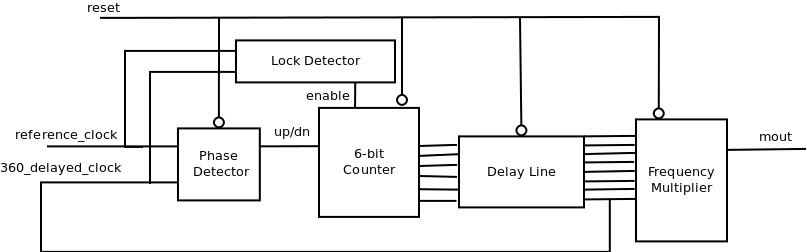
\includegraphics[width=150mm]{../Bilder/DIA_high_level.png}
        \caption{Overview of the system}
        \label{fig:system}
\end{figure}
\section{Block Level and Description}
\subsection{Phase Detector}
\subsection{Counter}
\subsection{Digitally Controlled Delay Line}
\subsection{Lock Detector}
\subsection{Frequency Multiplier}
\section{Simulation Result}
\subsection{Whole System Simulation}
\subsection{Phase Detector}
\subsection{Counter}
\subsection{Digitally Controlled Delay Line}
\subsection{Lock Detector}
\subsection{Frequency Multiplier}
\section{Risks and Delays}
\subsection{Counter}
\subsection{Digitally Controlled Delay Line}
\subsection{Frequency Multiplier}
\newpage 
\appendix 
\newpage

\addcontentsline{toc}{section}{References}
\begin{thebibliography}{99}
\bibitem{dll_clock}\textit{A Low-Power Digital DLL-Based Clock Generator in Open-Loop Mode - }
Behzad Mesgarzadeh, Atila Alvandpour \\
IEEE Journal of Solid-State Circuits. Vol. 44. No. 7. July 2009
\bibitem{lock_detect}\textit{A 62.5-625-Mhz Anti-Reset All-Digital Delay-Locked Loop - }
Shao-Ku Kao, Bo-Jiun Chen and Shen-Iuan Liu \\
IEEE Transations on Circuits and Systems - II: Express Briefs, Vol. 54 No. 7, July 2007

\end{thebibliography}
\end{document} 
%%% Local Variables: %%% mode: latex %%% TeX-master: t %%% End:
